\documentclass[12pt]{paper}
\usepackage[margin=1in]{geometry}
\usepackage{tikz}
\usetikzlibrary{plotmarks}

\title{Problem Set 4.1}
\author{Timothy Schwieg \and Daniel Noriega}
\begin{document}
\maketitle

Given: There is a market for housing with a range of quality
levels. New high-quality housing alternatives are produced by a
competitive industry with constant return to scale (i.e. constant
marginal cost). There is a fixed stock of existing houses
($H_{old}$ houses). Individuals differ in their level of income, but
have the same preferences.



Assumed: Quality of houses is assumed to be a normal good, so that as
income increases the quality choice increases. The number of
inhabitants for the market considered ($N_{pop}$) is assumed to be
greater than the number of existing houses ($H_{old}$), so that some
inhabitants must occupy new houses. Additional, all consumers are
assumed to have an income high enough so that they can afford renting
a house.  Since the producer of new houses exhibits a CRS function, it
is assumed to make no profits ($\Pi_{new} = 0$) in
equilibrium. Additionally, since it is given that new houses will be
``high quality'' houses, we assume that the derivative of the unit
cost of production function for new houses is smaller than the
hypothetical one for existing houses (i.e.
$UC'_{new} (q) < UC'_{old} (q)$). We interpret the unit cost of
increasing the quality in the context of maintenance frequency and
amenities provided. Maintenance such as heating is more expensive to
provide in older houses. We assume that they have lower unit cost to
provide in new houses compared to older houses.

\section{Part A}
Q: Describe the equilibrium to this model. Who would tend to live in
the new houses?
What will determine the price of the old houses
(which range in quality)?
\\

We assumed that $H_{old} < N_{pop}$. However, we have not made any
determinations on the consumers' income distribution. We will assume
that there exist two types of consumers, rich and poor. Let
$M_{rich} > M_{poor}$ and $N_{poor} + N_{rich} = N_{pop}$. Denote $M_x$
as the income of group $x$.
\\

$$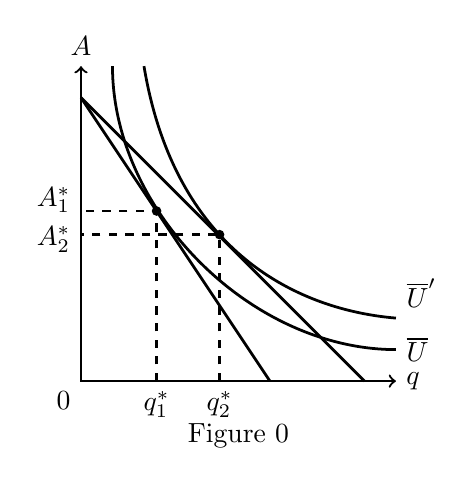
\begin{tikzpicture}[scale=0.4, line width = 1pt]

\draw[thick,<->] (0,10) node[above]{$A$}--(0,0)--(10,0) node[right]{$q$};

\node [below left] at (0,0) {$0$};

\filldraw (4.4,4.65) circle (3pt);
\draw[dashed] (4.4,0)--(4.4,4.65)--(0,4.65);
\node[below] at (4.4,0){$q_2^{*}$};
\node[left] at (0,4.5){$A_2^{*}$};

\filldraw (2.4,5.4) circle (3pt);
\draw[dashed] (2.4,0)--(2.4,5.4)--(0,5.4);
\node[below] at (2.4,0){$q_1^{*}$};
\node[left] at (0,5.75){$A_1^{*}$};

% \node [below] at (4,0) {$v_2^{*}$};
% \node [left] at (0,5) {$F_{1}^{*}$};
% \node [below] at (5,0) {$v_1^{*}$};
% \node [left] at (0,6.5) {$F_2^{*}$};

\node [below] at (5,-1){Figure 0};

\draw(0,9)--(9,0) node[right]{};
\draw(0,9)--(6,0) node[right]{};

% \draw[dashed](0,5)--(5,5)--(5,0);
% \draw[dashed](0,6.25)--(4.3,6.25)--(4.3,0);

\draw(1,10) ..controls (1,5.4) and (5.4,1) .. (10,1)
node[right]{$\overline{U}$};

\draw(2,10) ..controls (3,4) and (7,2.25) .. (10,2) node[above right]{$\overline{U}^{\prime}$};

\end{tikzpicture}$$

Consider the consumer's problem between the choice in the quality of
the house and some auxiliary good that bundles all other choices. As
the price of quality changes, a different quality is demanded. All of
these choices map out the demand for quality of a particular
individual. The individuals in the rich group have a higher
income. Since quality in houses is normal, the rich group has a higher
demand than the poor group.\newline

\textbf{Claim: Higher-income individuals tend to live in the new
  houses, and the relative price of old houses will depend on the
  relative scarcity of low-income individuals and existing houses.}\newline

Quality of houses are a normal good. For two different sets of income,
the individual with the higher income will have choose
a higher quality house. In equilibrium he will then occupy the higher
quality house. The poorer individual will occupy the lower quality
house, or the older house. We already established that
$H_{old} < N_{pop}$. Nonetheless, it could be the case that
$H_{old} > N_{poor}$. Some of the high income individuals would also
occupy existing houses, or that $H_{old}< N_{poor}$, so that low
income individuals occupy some new houses because old houses are
scarce relative to the low income population.
\\

\textbf{Case 1: $H_{old} > N_{poor}$}

In this case some high-income individuals will also occupy existing
houses. For a given level of income (high), individuals must be
indifferent between living in new and old houses. Consequently, old
houses' prices will increase until the marginal quality cost function
is tangent to the same level curve for the representative high income
individual. In the equilibrium, additionally, poor individuals' level
curve must be tangent to the same marginal quality cost curve for old
houses. Otherwise, either there would be utility improvement
opportunities and the allocation would not be a competitive
equilibrium, or some of the poor individuals would not occupy a
house. This case is shown below in Figure 1.
\\

\begin{figure}[h!]
  \centering
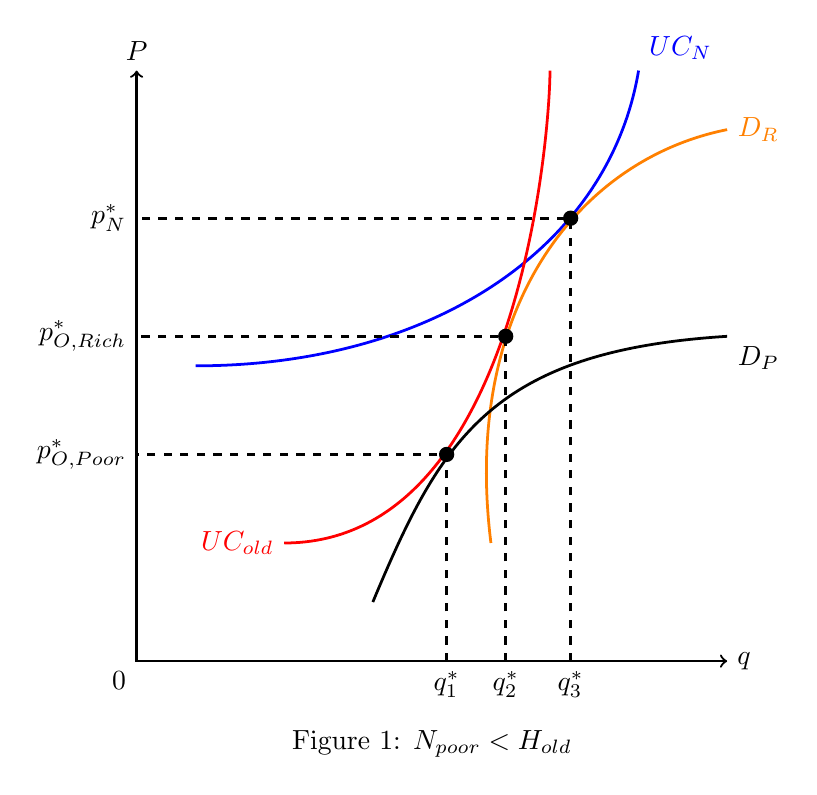
\begin{tikzpicture}[scale=0.75, line width = 1pt]

\draw[thick,<->] (0,10) node[above]{$P$}--(0,0)--(10,0) node[right]{$q$};

\node [below left] at (0,0) {$0$};

% \node [below] at (4,0) {$v_2^{*}$};
% \node [left] at (0,5) {$F_{1}^{*}$};
% \node [below] at (5,0) {$v_1^{*}$};
% \node [left] at (0,6.5) {$F_2^{*}$};

\node [below] at (5,-1){Figure 1: $N_{poor} < H_{old}$};

\draw [blue] (1,5) .. controls (5,5) and (8,7) .. (8.5,10)
node[above right]{$UC_{N}$};

\draw[red](2.5,2)node[left]{$UC_{old}$} .. controls (6.5,2) and (7,9)
.. (7,10);


\draw[orange] (6,2)..controls (5.5,6) and (7.5,8.5) .. (10, 9) node[right]{$D_R$};

\draw (4,1)..controls (5.15,3.75) and (6,5.25) .. (10, 5.5) node[below right]{$D_P$};


\filldraw (5.25,3.5) circle (3pt);
\draw [dashed] (5.25,0)--(5.25,3.5)--(0,3.5);
\node [left] at (0,3.5){$p_{O,Poor}^{*}$};
\node [below] at (5.25,0){$q_{1}^{*}$};


\filldraw (6.25,5.5) circle (3pt);
\draw [dashed] (6.25,0)--(6.25,5.5)--(0,5.5);
\node [left] at (0,5.5){$p_{O,Rich}^{*}$};
\node[below] at (6.25,0){$q_{2}^{*}$};


\filldraw (7.35,7.5) circle (3pt);
\draw [dashed] (7.35,0)--(7.35,7.5)--(0,7.5);
\node[left] at (0,7.5){$p_{N}^{*}$};
\node[below] at (7.35,0){$q_3^{*}$};



\end{tikzpicture}
\end{figure}

\newpage

\textbf{Case 2: $H_{old} < N_{poor}$}

In this case existing houses will be scarce relative to the low-income population so that some low-income individuals will have to live in new houses. In the equilibrium, high-income individuals will make a higher quality choice, while low-income individuals will make a lower quality choice and be indifferent between living in old and new houses. Therefore, old houses' prices will increase even further relative to case 1. This case is shown below in Figure 2.
\\

\begin{figure}[h!]
  \centering
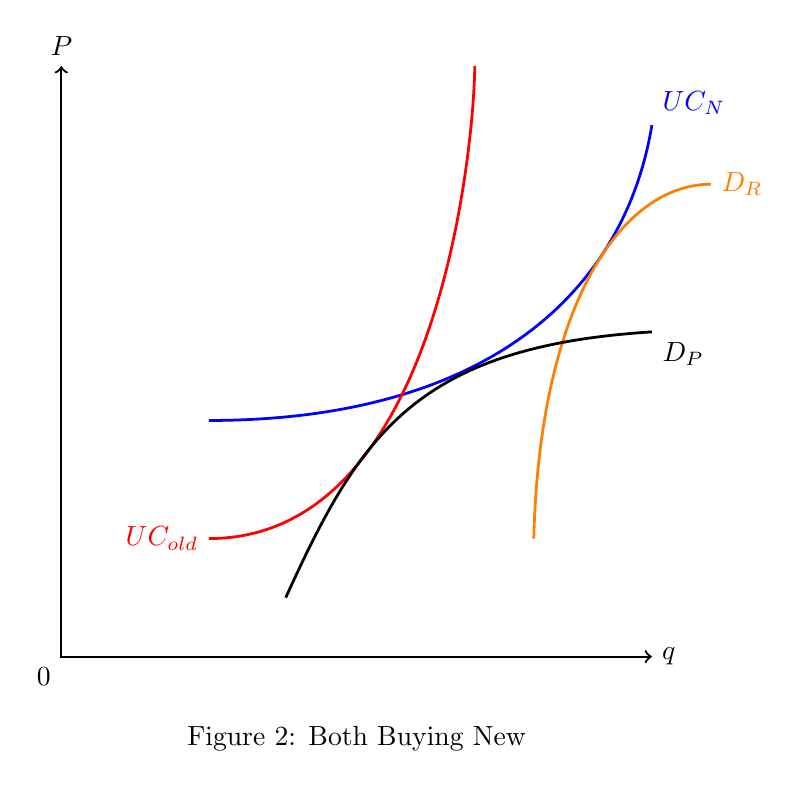
\begin{tikzpicture}[scale=0.75, line width = 1pt]

\draw[thick,<->] (0,10) node[above]{$P$}--(0,0)--(10,0) node[right]{$q$};

\node [below left] at (0,0) {$0$};

\node [below] at (5,-1){Figure 2: Both Buying New};

\draw[blue](2.5,4) .. controls (7,4) and (9.5,6) .. (10,9)
node[above right]{$UC_{N}$};

\draw[red](2.5,2)node[left]{$UC_{old}$} .. controls (6.5,2) and (7,9) .. (7,10);



\draw[orange] (8,2)..controls (8.1,6) and (9.5,8) .. (11, 8) node[right]{$D_R$};

\draw (3.8,1)..controls (5.05,3.75) and (6,5.25) .. (10, 5.5) node[below right]{$D_P$};

\end{tikzpicture}
\end{figure}

In both cases higher income individuals tend to live in the new houses. Additionally, we observe that the relative price of old houses will depend on the relative scarcity of old houses and low-income individuals.

\section{Part B}
Q: How would an increase in the income of a group of consumers (say
those in a given
range of the income distribution) affect housing
prices and the welfare of consumers at
the different levels of
income?
\\

Maintaining the assumptions made in part A we can further analyze what
could occur if any of the groups increased their income.
\\

Again, we will have to study two cases within this frame,
$N_{poor}<H_{old}$ (Case 1) and $N_{poor}>H_{old}$ (Case 2).
\\

\textbf{Case 1: $H_{old} > N_{poor}$}

An increase in the income of relative rich individuals
(i.e. $M_{rich}$) would further shift their level curve towards a
higher quality choices and increase the price of new houses. However,
since in the equilibrium higher income individuals still need to be
indifferent between new and some old houses (recall that some rich
individuals would occupy existing houses in this case), the relative
price of old houses for rich individuals would need to decrease. This
would require a shift downward of the unit cost curve for existing
houses (i.e. existing house owners' profits would decrease).  Since
the form of the curve of poor individuals has not changed, their
quality choice will be the same. Nevertheless, since the unit cost
curve for existing houses shifted down, the actual price for the same
quality choice would decrease, making lower income individuals better
off. This dynamic is shown below in Figure 3.
\\


\begin{figure}[h!]
  \centering
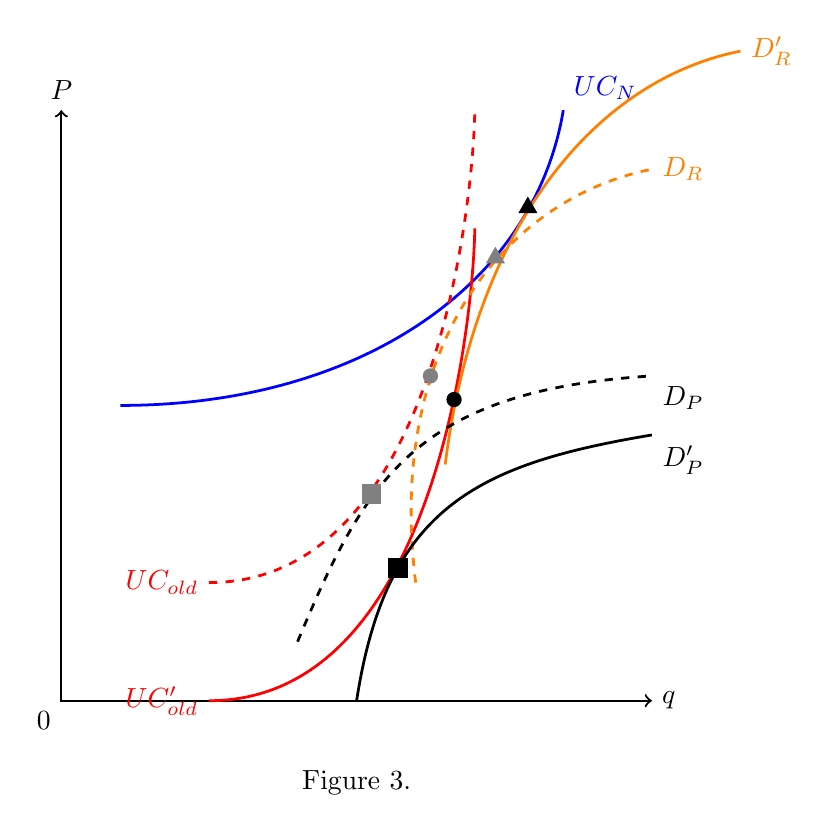
\begin{tikzpicture}[scale=0.75, line width = 1pt]

\draw[thick,<->] (0,10) node[above]{$P$}--(0,0)--(10,0) node[right]{$q$};

\node [below left] at (0,0) {$0$};

% \node [below] at (4,0) {$v_2^{*}$};
% \node [left] at (0,5) {$F_{1}^{*}$};
% \node [below] at (5,0) {$v_1^{*}$};
% \node [left] at (0,6.5) {$F_2^{*}$};

\node [below] at (5,-1){Figure 3.};

\draw [blue] (1,5) .. controls (5,5) and (8,7) .. (8.5,10)
node[above right]{$UC_{N}$};

\draw[red,dashed](2.5,2)node[left]{$UC_{old}$} .. controls (6.5,2) and (7,9)
.. (7,10);
\draw[red](2.5,0)node[left]{$UC_{old}'$} .. controls (6.5,0) and (7,7)
.. (7,8);


\draw[orange,dashed] (6,2)..controls (5.5,6) and (7.5,8.5) .. (10, 9) node[right]{$D_R$};
\draw[orange] (6.5,4)..controls (7,8) and (9,10.5) .. (11.5, 11) node[right]{$D_R'$};


\draw[dashed] (4,1)..controls (5.15,3.75) and (6,5.25) .. (10, 5.5)
node[below right]{$D_P$};

\draw (5,0)..controls (5.5,3.25) and (7,4) .. (10, 4.5) node[below right]{$D_P'$};


\node[mark size=3pt,gray] at (5.25,3.5) {\pgfuseplotmark{square*}};
\node[mark size=3pt] at (5.7,2.25) {\pgfuseplotmark{square*}};
% \draw [dashed] (5.25,0)--(5.25,3.5)--(0,3.5);
% \node [left] at (0,3.5){$p_{O,Poor}^{*}$};
% \node [below] at (5.25,0){$q_{1}^{*}$};


\filldraw[gray] (6.25,5.5) circle (3pt);
\filldraw (6.65,5.1) circle (3pt);
% \draw [dashed] (6.25,0)--(6.25,5.5)--(0,5.5);
% \node [left] at (0,5.5){$p_{O,Rich}^{*}$};
% \node[below] at (6.25,0){$q_{2}^{*}$};


\node[mark size=3pt,gray] at (7.35,7.5) {\pgfuseplotmark{triangle*}};
\node[mark size=3pt] at (7.9,8.35) {\pgfuseplotmark{triangle*}};
% \draw [dashed] (7.35,0)--(7.35,7.5)--(0,7.5);
% \node[left] at (0,7.5){$p_{N}^{*}$};
% \node[below] at (7.35,0){$q_3^{*}$};



\end{tikzpicture}
\end{figure}


Additionally, within this case, it is possible that the income of poor
individuals increased (i.e. $M_{poor}$), so that
$M_{rich}>New M_{poor}>Past M_{poor}$. In this case, although the
quality choice of poor individuals would tend to increase, causing an
increase in the price of old houses, there would be no shift in the
old houses' unit cost curve (i.e. $C_{old} (q)$). Which would indicate
that overall, existing house producers (or owners, since they are
already build) would make a similar "profit". Nonetheless, one could
imagine that additional income levels could be introduced in the
model, as well as additional unit cost of production curves. In this
case, shifts in unit cost curves could occur for certain income level
increases (similar to what occurred in Figure 3 for an $M_{rich}$
increase), but one would expect that since they tend to affect only
cheaper alternatives, the overall effect on welfare would be reduced
as the affected income level is poorer.
\newpage

\textbf{Case 2: $H_{old} < N_{poor}$}

In this case, if the $M_{rich}$ increases, their quality choice (and
the consequent housing price) would increase, but it would move along
the fixed unit cost curve for new houses (recall $\Pi_{new}=0$ and their
marginal cost is constant). Nonetheless, it would have no effect on
lower-income population's welfare.  On the other hand, if there was an
increase in $M_{poor}$ so that $M_{rich}>New M_{poor}>Past M_{poor}$,
lower-income individuals would shift their choices towards higher
qualities. Since poor individuals must be indifferent between new and
old houses in the equilibrium, there will be a shift downward in the
existing houses' unit cost curve. Overall, the welfare of poor
individuals would increase, as the price that they would have to pay
for the same quality choice would decrease. This is shown below in
Figure 4.
\\


\begin{figure}[h!]
  \centering
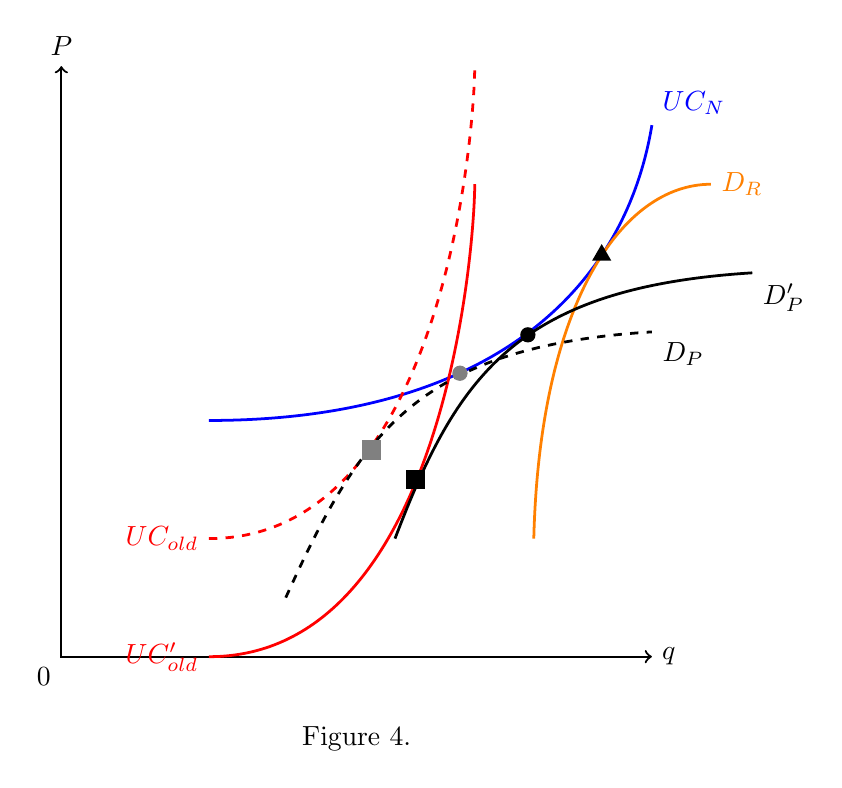
\begin{tikzpicture}[scale=0.75, line width = 1pt]

\draw[thick,<->] (0,10) node[above]{$P$}--(0,0)--(10,0) node[right]{$q$};

\node [below left] at (0,0) {$0$};

\node [below] at (5,-1){Figure 4.};

\draw[blue](2.5,4) .. controls (7,4) and (9.5,6) .. (10,9)
node[above right]{$UC_{N}$};

\draw[red,dashed](2.5,2)node[left]{$UC_{old}$} .. controls (6.5,2) and (7,9) .. (7,10);
\draw[red](2.5,0)node[left]{$UC_{old}'$} .. controls (6.5,0) and (7,7) .. (7,8);


\draw[orange] (8,2)..controls (8.1,6) and (9.5,8) .. (11, 8) node[right]{$D_R$};

\draw[dashed] (3.8,1)..controls (5.05,3.75) and (6,5.25) .. (10, 5.5)
node[below right]{$D_P$};

\draw (5.65,2)..controls (6.7,4.75) and (7.7,6.25) .. (11.7, 6.5)
node[below right]{$D_P'$};


\node[mark size=3pt,gray] at (5.25,3.5) {\pgfuseplotmark{square*}};
\node[mark size=3pt] at (6,3) {\pgfuseplotmark{square*}};
% \draw [dashed] (5.25,0)--(5.25,3.5)--(0,3.5);
% \node [left] at (0,3.5){$p_{O,Poor}^{*}$};
% \node [below] at (5.25,0){$q_{1}^{*}$};


\filldraw[gray] (6.75,4.8) circle (3pt);
\filldraw (7.9,5.45) circle (3pt);
% \draw [dashed] (6.25,0)--(6.25,5.5)--(0,5.5);
% \node [left] at (0,5.5){$p_{O,Rich}^{*}$};
% \node[below] at (6.25,0){$q_{2}^{*}$};


\node[mark size=3pt] at (9.15,6.8) {\pgfuseplotmark{triangle*}};
% \draw [dashed] (7.35,0)--(7.35,7.5)--(0,7.5);
% \node[left] at (0,7.5){$p_{N}^{*}$};
% \node[below] at (7.35,0){$q_3^{*}$};


\end{tikzpicture}
\end{figure}

\newpage
Income increases for groups that are indifferent between the new and
existing houses, have larger welfare effects than the groups that are
only consuming one type of household. 

\section{Part C}
Q: What would happen if the government replaced a number of the oldest
houses with new
ones through a process of urban renewal? Who would
gain from that? Why? Could
some people lose? How would the answers
differ if individuals owned versus rented
their housing?
\\

In our simplified model, there are four representative agents
involved: poor individual, rich individual, old house owner and new
house provider. In equilibrium, given our framework, rich individuals
are always either indifferent between occupying an old and a new house,
or only living in new houses. Since the new houses provider exhibits
CRS, the marginal cost of producing a new house would not increase,
and therefore, rich individuals would never be better nor worse off.
New house providers by definition, must have $\Pi=0$, and therefore,
would not be affected by the replacement process either. They would
simply provide more houses at the same marginal cost without any
profits.  Old house owners, in general, will be worse off since they
are earning a profit, and presumably they will not be earning one
after their house is replaced. However, this would depend on the
actual replacement mechanism (i.e. how much are they receiving?), so
it is uncertain whether they would be better off.

If poor individuals had been indifferent between living in old and new
houses (recall Part A - Case 2), they would not be affected by the
replacement process either. Conversely, if they were using only old
houses (recall Part A - Case 1), once a house is replaced, a poor
individual will have to afford another house that he decided not to
afford when she had the alternative. Therefore, the poor individual
will have to make a choice that was not maximizing their utility
before, which could only make them worse off. If she had to chose a
quality/price combination on the new houses unit cost curve, she would
chose a lower quality product (recall $C'_N(q)<C'_O(q)$).
\\

If individuals owned their houses, however, the initial ``profit''
that they were earning (recall that the unit cost curve for old houses
was shifted upwards once new houses were introduced) could be either
maintained, increased or destroyed during the replacement
process. Depending on the actual replacement mechanism they could be
either indifferent, better, or worse off. If they had to make any
payments, for example, they could be worse off if those are not
out-weighted my the benefits in quality/price they would receive from
the new house, but that they decided not to afford before. Conversely,
if they received a house that is strictly better quality/higher price
at virtually no cost, they would be better off.
\\

\section{Part D}
Q: Now assume that other aspects of life differ across houses in that
the level of city services
(e.g. police protection) differs across
houses with the lower quality homes also receiving
less police
protection. How would a policy that mandated equal levels of services
across
areas affect outcomes? Who would gain from such a policy?
Assume the amount of
service is set equal to that of the highest
quality homes, and that any additional spending
is financed by lump
sum taxes on consumers.
\\

For simplicity-sake, we will assume that in this case consumers are
only renting houses.

When a consumer rents a house, he now rents two goods. The quality of
the house is bundled with the police protection alongside it. For each
quality of house there is an associated level of police protection. At
first, allow this quality of police protection to vary directly with
the quality of house. Higher quality houses have higher quality police
protection. Assume that this equilibrium fits the base graphs above.

Now the level of the police protection is no longer allowed to
vary. Each quality house is now given the same protection as the
highest quality houses were receiving before. Houses of lower quality
now are relatively better, since the level of bundled police
protection good is now higher. As lower quality houses are
relatively better, people of all income levels demand them more. This
means that lower quality houses are demanded more, and income of both
groups drops by paying for this police force. This reduces the demand
for all houses, and as housing quality is a normal good, biases both
groups towards lower quality houses.
\\


The rich group of people were consuming new houses with the
highest level of police protection. Now they have less income
available to them as they are being taxed as consumers. This leads
them to consume lower quality houses. If there are rich people
consuming the older houses, they change their consumption of older
houses to be indifferent to the new houses. The group consuming the
new houses is strictly worse off as it has less income, lower quality,
and equal police protection. As they are indifferent to the group
(possibly) consuming old houses, all rich consumers are made worse off.
\\

There is now relatively less cost to renting a lower quality
house. The cost of lowering quality is no longer less police
protection and lower quality. Poor people also have less income
available to them since they are taxed. These two factors lead to poor
people choosing a lower quality of house. Note that poor people do not
choose the high level of police protection in the previous
equilibrium. This tells us that they prefer higher quality of house to
higher police protection, at their current level of consumption. Poor
consumers are therefore worse off after the policy, as they were
gaining an advantage from the lower quality homes having low police
protection. This advantage was caused by them being less willing to
pay for the police protection than the richer group, and thus
benefiting more from police protection being reduced.
\\

The land-lords of the old houses would gain from the policy. A lower
quality house now has more demand for it, and therefore a higher
rental price. This increases the returns to the land-lords and makes
them strictly better off. Makers of the new homes continue to produce
at zero profits and are unchanged by the policy.

\end{document}